\section{Evaluation}

\subsection{Evaluation of the models}
To evaluate our model, we have decided to model the paediatric pneumonia guideline \parencite{RepublicofKeny2016}. As we have a strict time limitation it is better for us to evaluate a respiratory condition, as we have already worked with a respiratory condition in asthma. There is quite a lot of work for software developers to learn a new clinical guideline, so we save a lot of time when the concepts are similar.

In figure \ref{fig:PneumoniaEntityGraph} we have modelled the entity model of the paediatric pneumonia guideline \parencite{RepublicofKeny2016}. We see that both guidelines have a history part, where the patient or dependants can tell something about the condition of the patient. Both guidelines also have an examination part where the clinician looks for several symptoms. The symptoms are a bit different from paediatric possible asthma guideline, but they have several symptoms in common. Wheeze is something the clinician has to be aware about. If the patient is wheezing, the patient should be treated according to the paediatric possible asthma guideline instead.

The management part is also quite similar to the paediatric possible asthma guideline. The patient and dependants will be given some advise concerning the medical condition of the patient. If the pneumonia is severe, or the patient has lower chest wall indrawing and the patient cannot be reviewed within 48 hours, the patient should be admitted into the hospital. The medication is quite similar to the paediatric possible asthma guideline. For pneumonia there are fewer medications, but both guidelines have treatment with antibiotics and oxygen.

The big difference is the diagnostic part. For the paediatric possible asthma guideline, there is only one medical condition described. However, for the paediatric pneumonia guideline patients with tuberculosis or HIV will receive a different treatment. We have not modelled the treatment for pneumonia patients with HIV or tuberculosis as they are separate guidelines. But we need to identify such patients and refer to their respective guidelines. The same goes for asthma. Wheezing patients needs to be identified for asthma treatment.

To support several conditions, we have used inheritance on the diagnosis vertex. A new problem occurs as how should we model tuberculosis, no tuberculosis and that we don't know if the patient has tuberculosis? Earlier on, we used the open world principle for the symptoms. If the vertex doesn't exist, we haven't done the examination for the symptom and we don't know if the patient has it or not. The same goes for diagnosis. If the vertex is not there, we need to clarify if the patient has tuberculosis. To model the situation where we know that the patient hasn't tuberculosis, we have introduced the diagnosis "no tuberculosis". An alternative solution could be to introduce an attribute "status". The attribute could hold information about the patient evidently has the condition, evidently don't have the condition and if it is not clarified. A fourth status could be if the condition is recurring.

\begin{figure}[h!]
	\label{fig:PneumoniaEntityGraph}
	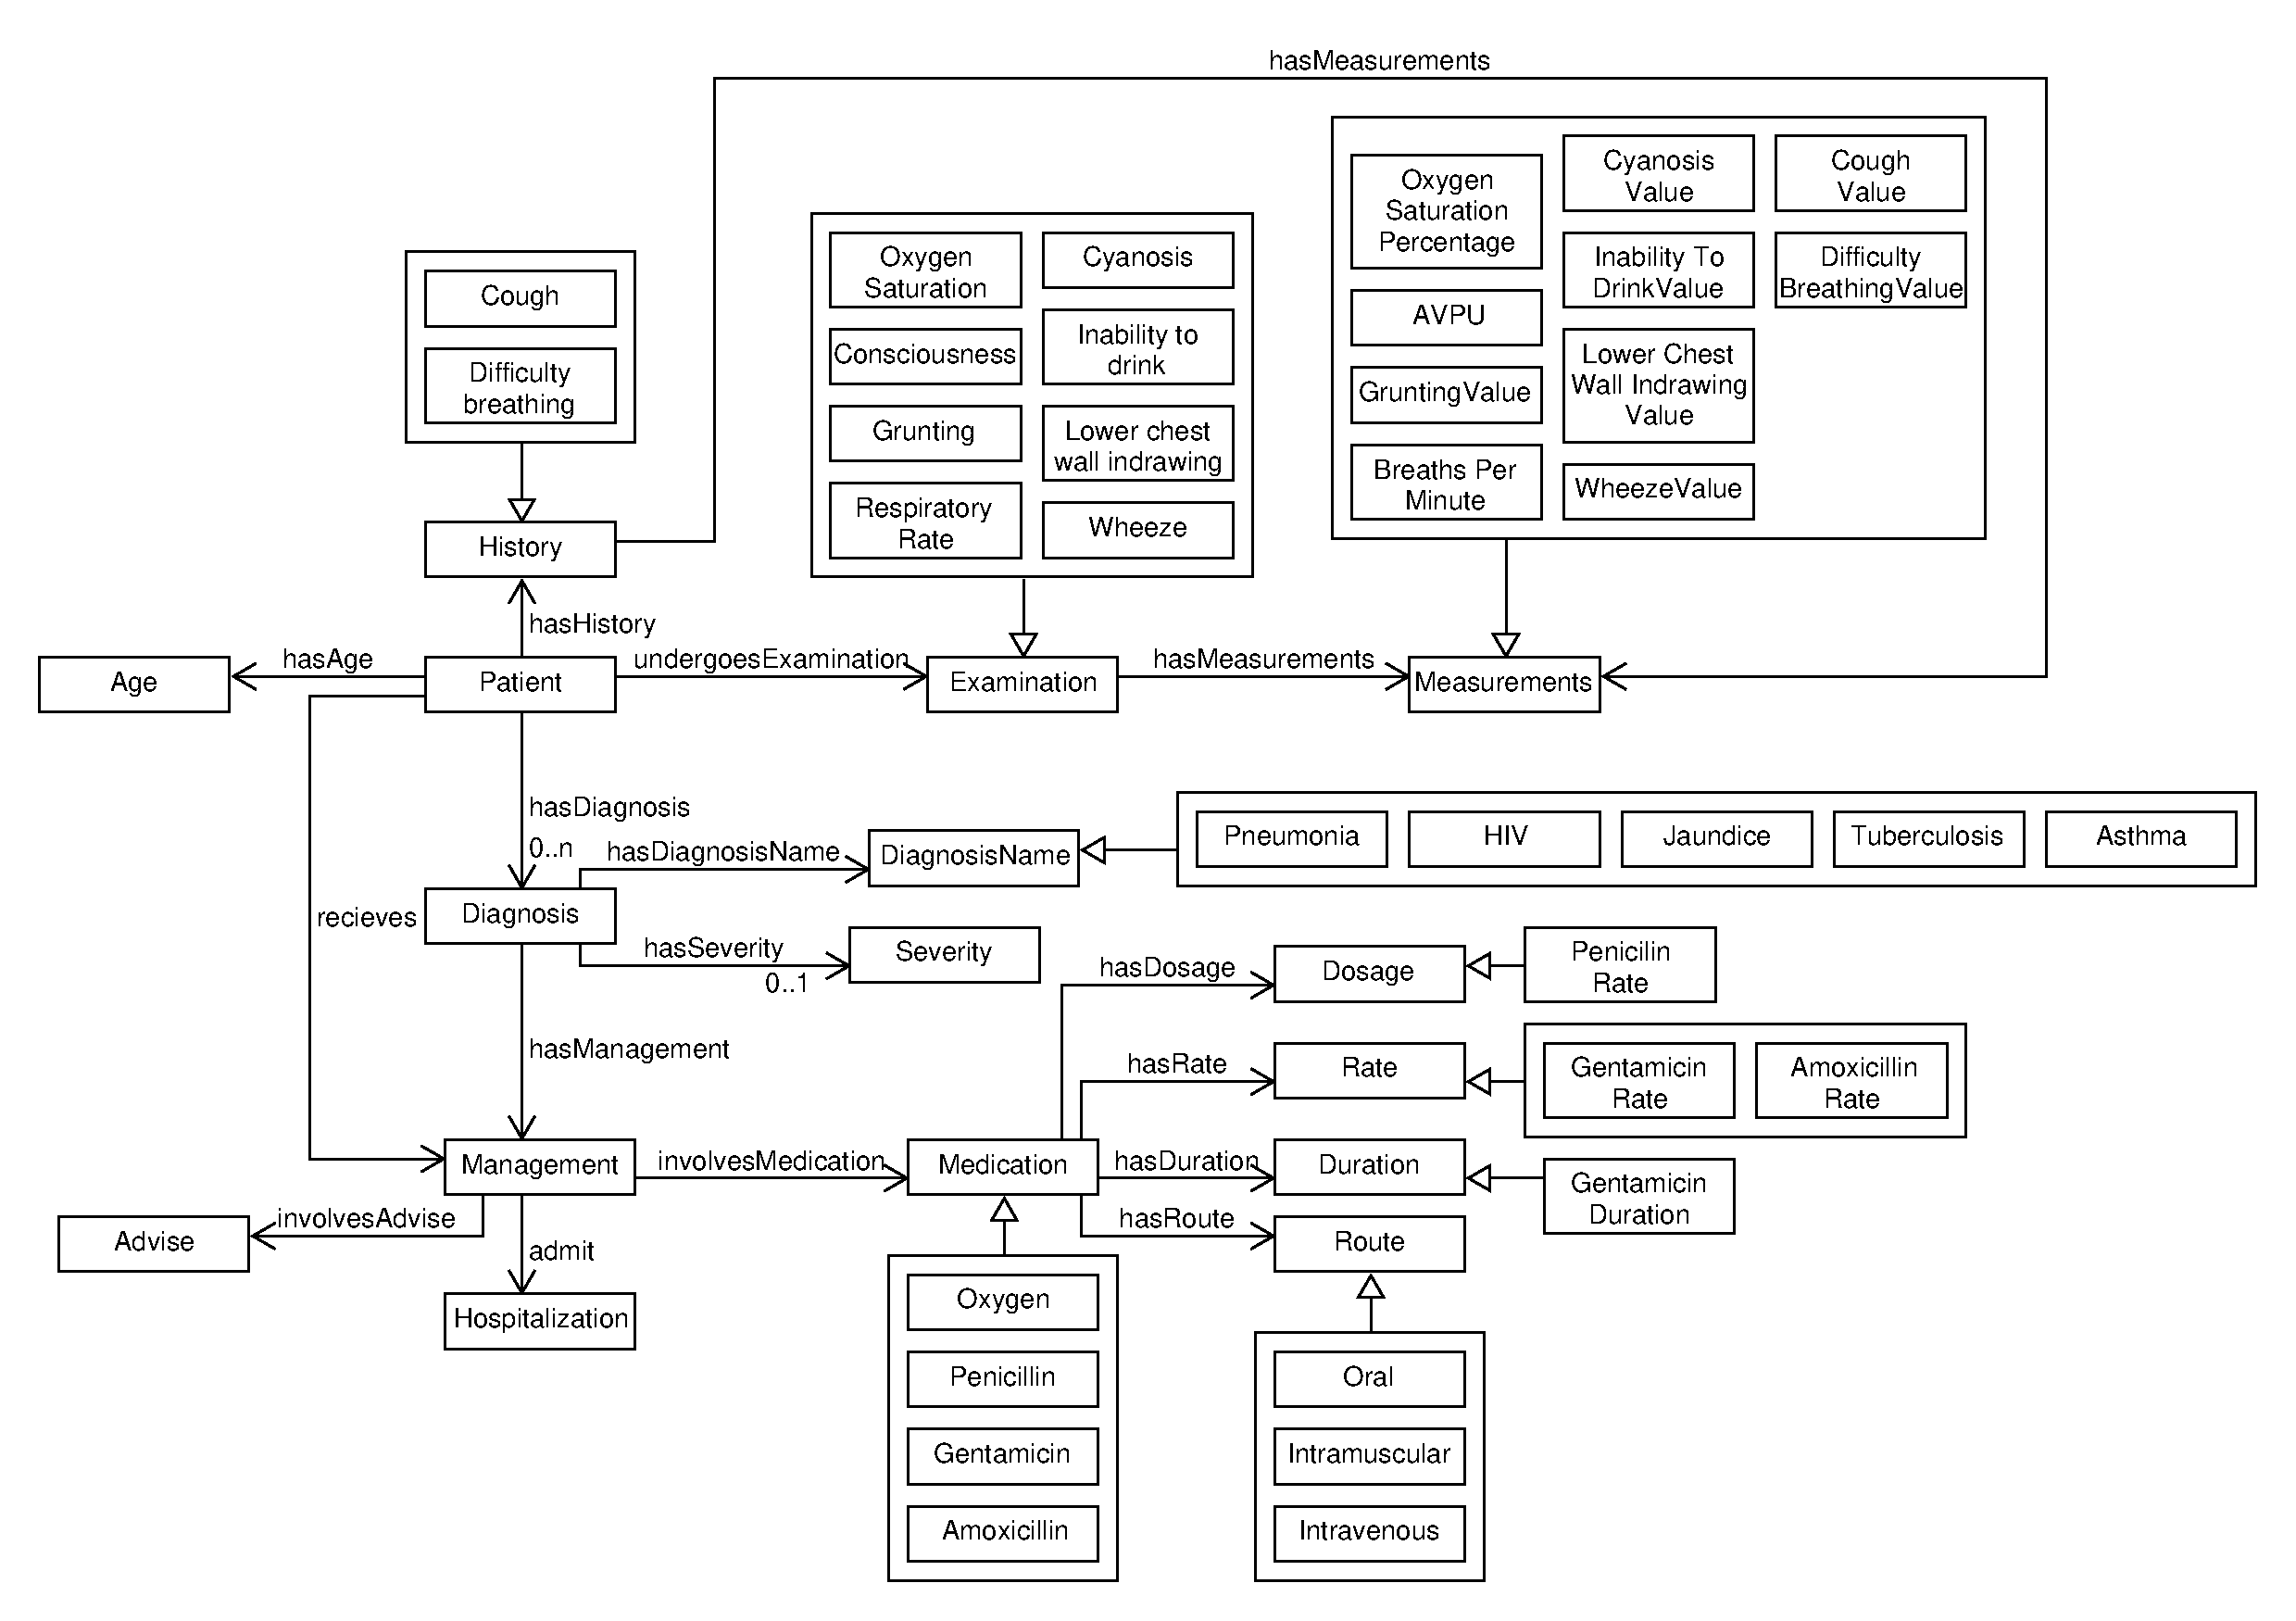
\includegraphics[scale=0.33]{PneumoniaEntityGraph}
	\caption {We are showing that our model is general enough to represent other CPGs. Here we have modelled the paediatric pneumonia guideline \parencite{RepublicofKeny2016}}
\end{figure}

To evaluate the workflow model in figure \ref{fig:WorkflowGraph}, we do like we did for the paediatric possible asthma guideline \parencite{RepublicofKeny2016}. We see the guideline in combination with the entity entity and the workflow model. The paediatric possible asthma guideline \parencite{RepublicofKeny2016} has an assessment part, where we look for patient older than 60 days, cough or difficulty breathing. If he has those symptoms and does not wheeze, we continue looking for other pneumonia symptoms. In the diagnostic part we strengthen our assumption of pneumonia, we set the severity of the diagnosis and we further keep in mind that if the the patient is wheezing he should be given the asthma treatment. Pneumonia patients with HIV or tuberculosis should be referred to specific guidelines for those condition combinations \parencite{RepublicofKeny2016}. In the management part, some patients get admitted into the hospital. The management further has an advise for review within 48 hours. The patients condition is then evaluated either on the hospital for admitted patients, or in a review within 48 hours for other patients. We can conclude with that the workflow model  also covers the paediatric pneumonia guideline \parencite{RepublicofKeny2016}.

In figure \ref{fig:PneumoniaPneumoniaIntegratedEntityWorkflowModels} we demonstrate an instance of the entity model working together with an instance of the workflow model. The patient goes through assessment, diagnosis, management and evaluation. As the patient has jaundice, he won't receive penicillin treatment. As the the pneumonia is severe, the treatment will be evaluated at the hospital and schedule for review is unnecessary. 
\begin{figure}[h!]
	\label{fig:PneumoniaPneumoniaIntegratedEntityWorkflowModels}
	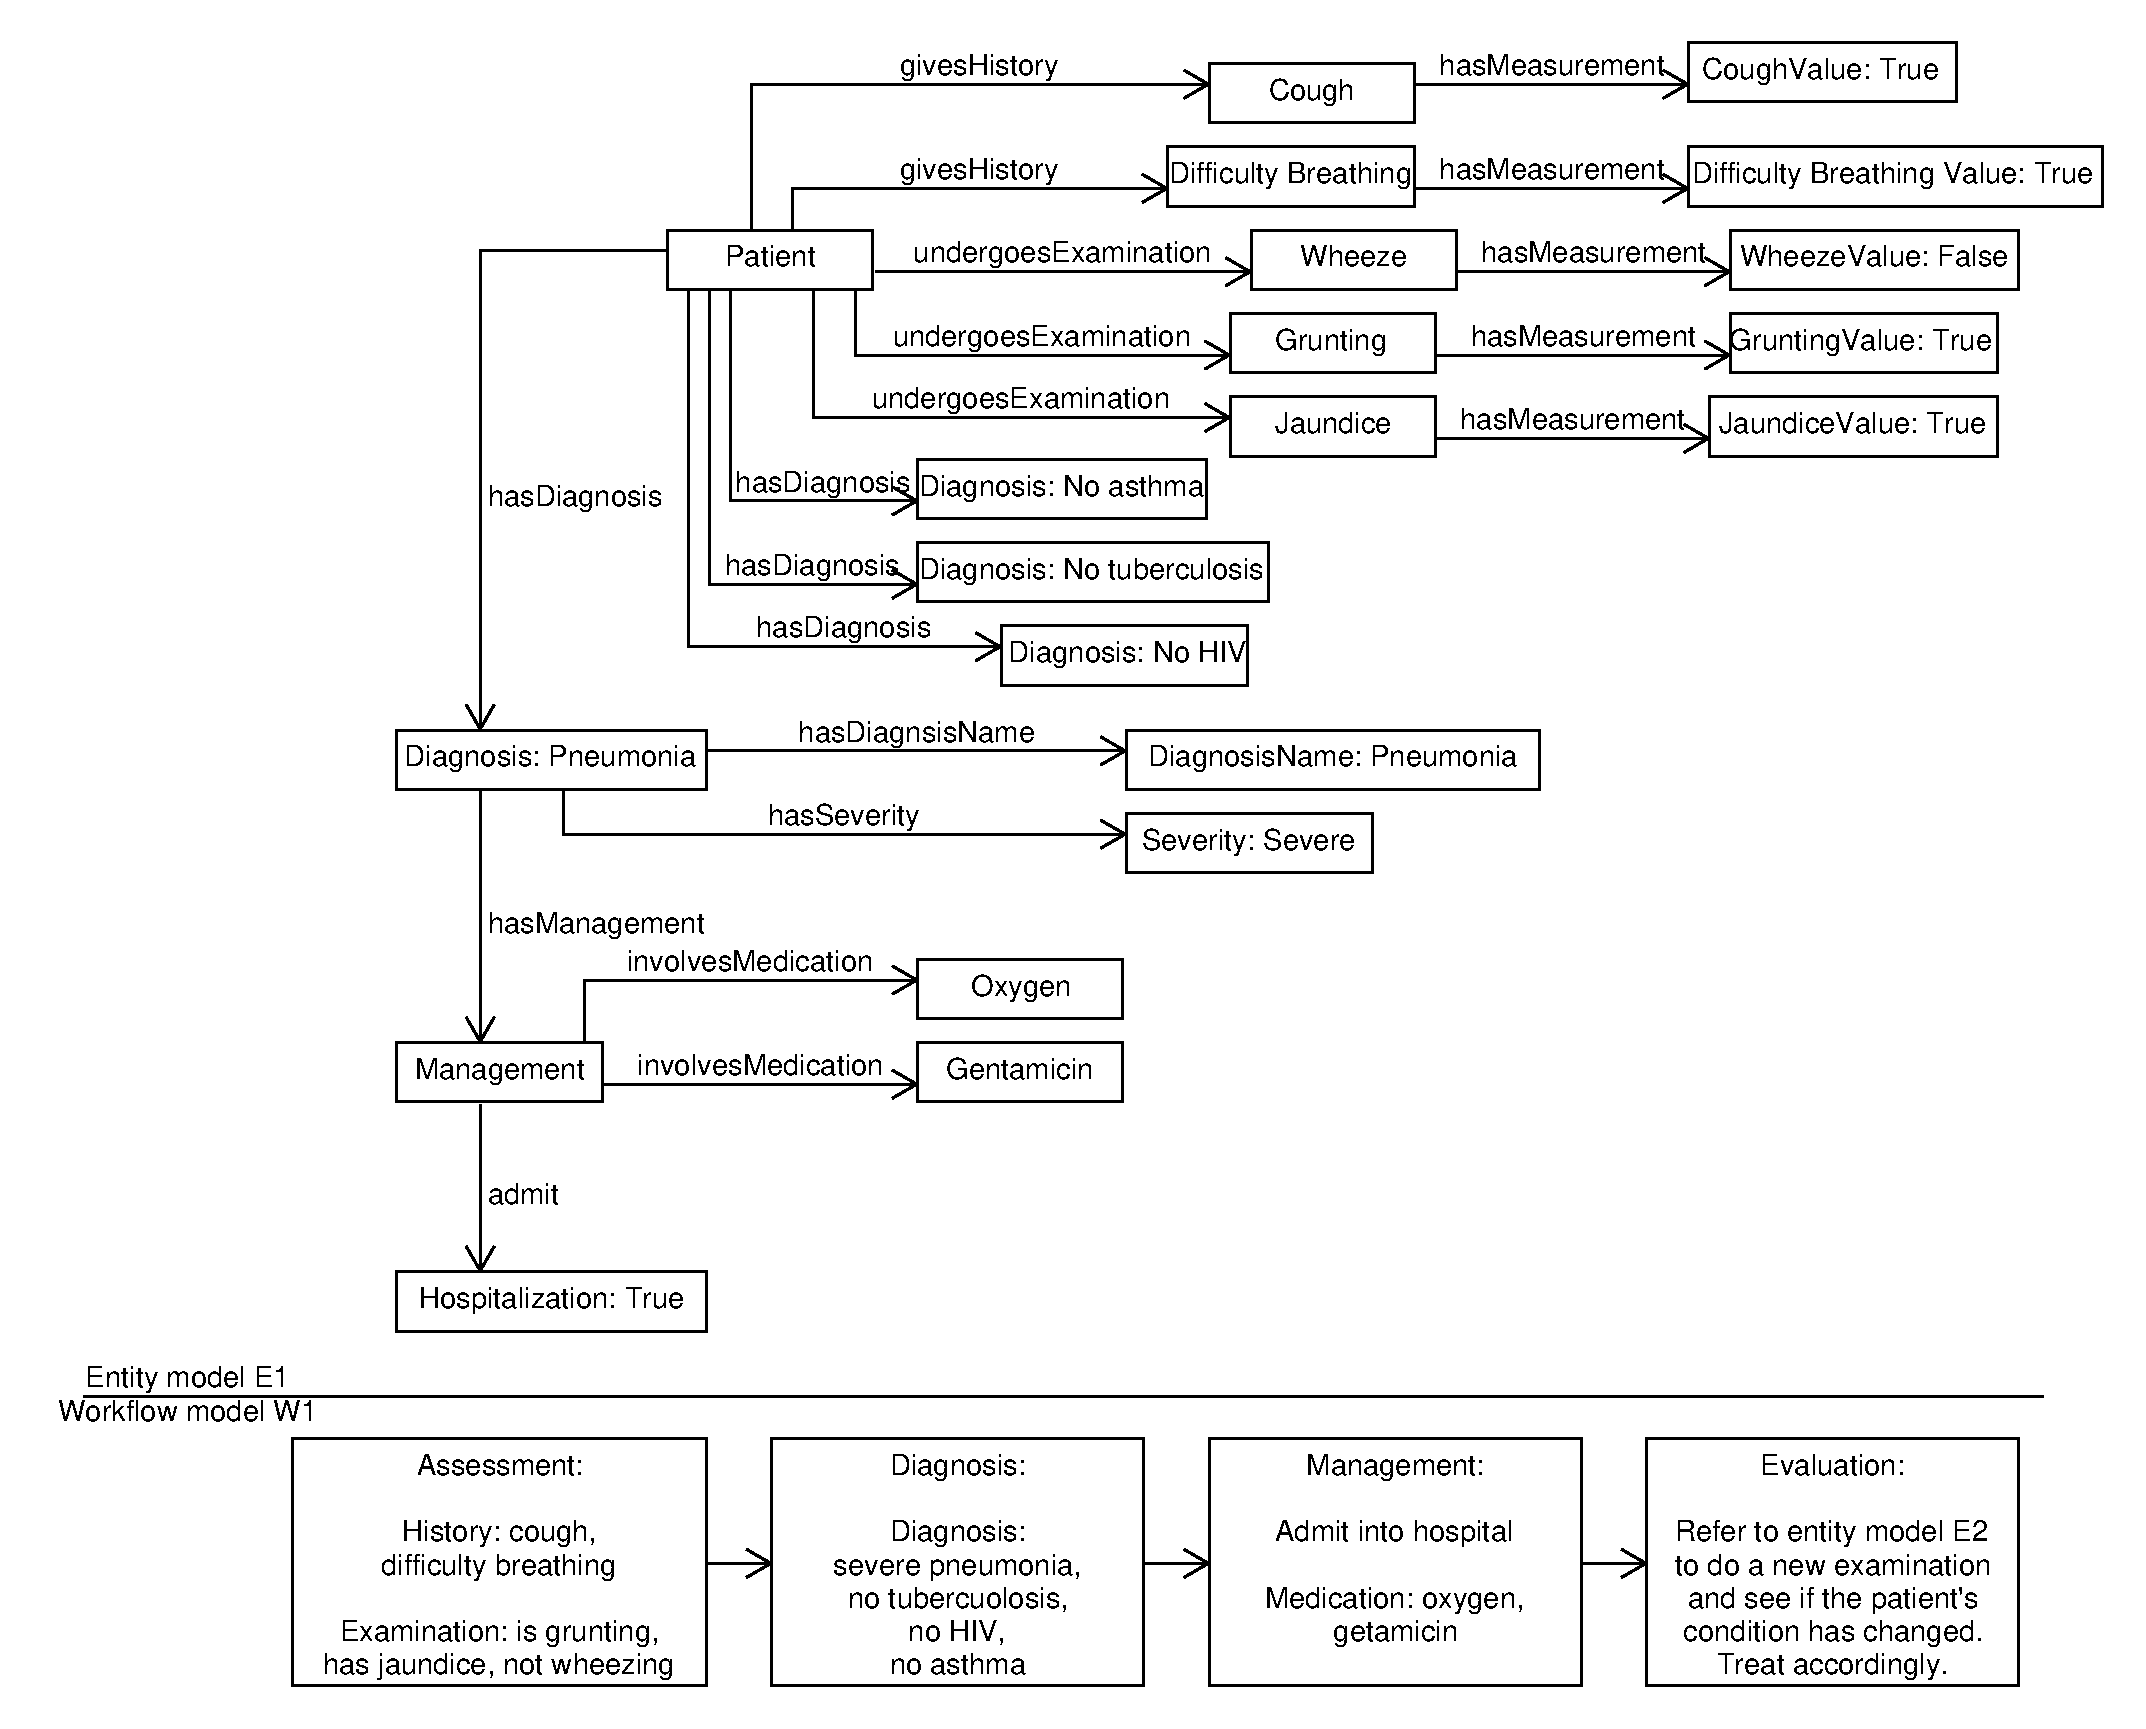
\includegraphics[scale=0.4]{PneumoniaIntegratedEntityWorkflowModels}
	\caption {We are showing out entity model working together with the workflow model for paediatric pneumonia guideline \parencite{RepublicofKeny2016}}	
\end{figure}

After the evaluation, we see that we have modified the entity and workflow models to support both pneumonia and asthma in paediatric medicine. It is likely that further modification and expansion of the entity model is needed when modelling other CPGs. However, we see that we have identified reusable elements of the guidelines, and our models can work as a stepping stone for guideline formalization standardisation.


\subsection{Evaluation of the application}
The evaluation of the application was done with clinicians.	Two medical doctors and two specialist nurses. Both of the specialist nurses are employees at the polyclinic for pulmonary diseases at Haukeland University. One of the nurses is a specialist in sleep apnea, and his master thesis was writing clinical guidelines for sleep apnea. The other nurse is a specialist in asthma, but in adult medicine.

The evaluation method was a combination of the cognitive walkthrough and usability test in controlled environment, with follow-up questions. In detail what we did was, the clinicians would be asked to play the most difficult level of the game, speak what they are thinking when playing the game and manoeuvring in the application. Topics to discuss would occur when the clinicians had to think out loud. The master student would observe and take notes when problems and confusions occurred, or that the clinician expressed emotions such as joy, excitement or disappointment.

\begin{enumerate}
	\item Can the application be a useful learning tool for medical students, nurses and doctors?
	\begin{enumerate}
		\item Very useful indeed. Would be nice to take a test after a lecture about asthma or after having read about asthma to see how much I have learnt and remember. A quiz is far more fun than a check list in paper format. The application is also good for scalability, as you can train a lot of clinicians without adding any resources. Also great if a course leader can see the progress or the level of his students.
		\item Absolutely useful, and I feel I have learnt a lot by just doing this quiz. The nurse found the game to be very engaging, cheering when getting a correct answer. 
	\end{enumerate}
	\item How is the flow of the questions? Is the idea of scenarios where we go from assessment, diagnosis, management and follow-up a good approach?
	\begin{enumerate}
		\item Happy with the float and the use of scenarios.
		\item Very happy with the float, being able to follow the patient from the start to the end of the treatment.
	\end{enumerate}
	\item Did we manage to present the important elements of the asthma guideline?
	\begin{enumerate}
		\item Don't know the asthma guideline well enough to answer that.
		\item Don't know the paediatric asthma guideline well enough to answer that.
	\end{enumerate}
	\item Is the detail level the element to adjust for the difficulties of questions?
	\begin{enumerate}
		\item Yes, but would like to have an even harder level with more details.
		\item Yes, it seems like a right approach. The target group of users is relevant here, that this is meant for the emergency clinic.
	\end{enumerate}
	\item How are the answer key explanations?
	\begin{enumerate}
		\item 
		\item I like how the measurements corresponds and are calculated with the scenario and the patient they are presented with. The answer key explanations gives relevant answers to the questions asked.
	\end{enumerate}
\end{enumerate}

Quality of questions
\begin{itemize}
	\item The assessment, none of the distractions is a wrong answer. Even though wheeze is what we are looking for.
	\item When asking for salbutamol dosage, it is relevant to know where and in which stage of the treatment it is being given. Also saying something about rate or duration can help clarify that.
	\item Very nice that we in some questions change the way we ask. Sometimes we give a diagnosis and asks which symptoms identifies it. Then we give some symptoms and then ask about the diagnosis.
	\item In the assessment part of the scenarios, we tell that clinical encounter happens at the emergency clinic. But we should find a way to amplify it even more, as one of the test persons missed that detail.
	\item Descriptions such as "age > 12 months" is hard for clinicians to read. We should avoid using logical operands.
	\item "Recurrence of asthma" is unclear. Who says that it is recurrent? Is it recurrent when the patient is in the emergency clinic? Does the patient tell that it is recurrent? Is it in the journal?
	\item We have a trick question and we should avoid those. We ask what is not the right way to administer salbutamol to a patient. The answer is oral. The clinician thought the right answer could be one of the other alternatives as an oral version of salbutamol doesn't exist.
\end{itemize}

User interface and game experience
 \begin{itemize}
 	\item All the clinicians were very positive to the multiple-try with hint approach. When they give a wrong answer, they get a new chance to revise the question and correct their answer.
 	\item When the clinicians answer a question incorrectly, they are presented with a "learn more" button. When they click on this button they get presented with an answer key explanation. When they click on "next" they get very surprised and disapointed that were taken to the next question and don't get the chance to get the question right.
 	
 	Here the specialist in asthma had a very interesting suggestion. When she clicks on "learn more", she want an explanation of why that suggestion was wrong or in which situations that answer would have been correct. Then she want to try again to collect the reward. She was noticeably disappointed at the summary when she saw that she was penalized hard for clicking "learn more".
 	\item The clinicians wanted a link or a button to display the clinical guidelines in the screen they were presented with the answer key explanation. Then they can read and learn more.
 	\item The clinicians noticed that they didn't have to remember details from the previous question before they answered the next. That was something they appreciated.
 	
\end{itemize}

\textcolor{red}{Er nødt til å skrive et sammendrag her, sånn at vi klarer å treffe forskningsspørsmålene mye bedre. Skal ha evaluering med en eller to leger på søndag, så det gir mening å forme og spisse dette avsnittet litt mer etter det møtet.}

\section{Limitations of the model}
\begin{itemize}
	\item Can't ask questions like "what are the symptoms for severe asthma?"
	\item Difficult to ask what NOT to do. If the vertex doesn't exist, only an empty string gets returned. Can only be used were we actually have written "don't admit to the hospital" as an example with hospitalization.
	\item \textcolor{purple}{TODO Yngve: Graph QL?}The inheritance makes it difficult to generalize some questions. We can't make a template which asks about the Rate a medicine should be taken with. We need to specifically ask for that medicine. To be able to ask for a general medicine, one solution can be to introduce a new tag which compares the substring of the type of the vertex. Another solution is to use the meta model and not the instance model. We don't use inheritance on diagnosis because of this.
	\item To avoid the problem described in the previous point, we don't use inheritance on Diagnosis. A limitation here is that  
	a patient can only have one diagnosis.
\end{itemize}
	

